\documentclass[dvipdfmx]{jsarticle}

\usepackage{ascmac}
\usepackage{url}
\usepackage[dvipdfmx]{hyperref}
\usepackage{pxjahyper}
\usepackage[dvipdfmx]{graphicx}
\usepackage{float}
\usepackage{listings,jlisting}

\hypersetup{
  colorlinks=true,
  urlcolor=cyan,
  linkcolor=black
}

\lstset{
  basicstyle={\ttfamily},
  identifierstyle={\small},
  commentstyle={\smallitshape},
  keywordstyle={\small\bfseries},
  ndkeywordstyle={\small},
  stringstyle={\small\ttfamily},
  frame={tb},
  breaklines=true,
  columns=[l]{fullflexible},
  numbers=left,
  xrightmargin=0zw,
  xleftmargin=3zw,
  numberstyle={\scriptsize},
  stepnumber=1,
  numbersep=1zw,
  lineskip=-0.5ex
}


\begin{document}

\section{実験目的・課題}
以下の3つの課題を行う。
\begin{itemize}
  \item 課題1
        \begin{itemize}
          \item 数値微分の方法を理解する
          \item $sin(x)$を微分するプログラムを作成する
          \item 幅を変更し精度が変化することを確認する
        \end{itemize}
  \item 課題2
        \begin{itemize}
          \item 数値積分の方法を理解する
          \item 円の面積を求めるプログラムを作成する
          \item 分割数を変更し精度が変化することを確認する
        \end{itemize}
  \item 課題3
        \begin{itemize}
          \item 上記以外の微分法・積分法について調査しプログラムを実装する
        \end{itemize}
\end{itemize}

\section{実装方法}

\subsection{課題1}

式\ref{bibun1}によって関数$f(x)$の微分は定義される。
\begin{equation}
  f'(x) = \lim_{h \to 0} \frac{f(x+h)-f(h)}{h}
  \label{bibun1}
\end{equation}
しかし、計算機では極限の計算はできない。そのため、
hに微小量を設定して近似して解を得る。

微分を計算する差分のとり方は3つあり、それぞれ
前方差分(式\ref{forward})、後方差分(式\ref{backward})、中心差分(式\ref{central})である。
\begin{equation}
  f'(x) \simeq \frac{f(x+h)-f(x)}{h}
  \label{forward}
\end{equation}
\begin{equation}
  f'(x) \simeq \frac{f(x)-f(x-h)}{h}
  \label{backward}
\end{equation}
\begin{equation}
  f'(x) \simeq \frac{f(x+h)-f(x-h)}{2h}
  \label{central}
\end{equation}

$f(x)$の$x=a$まわりでのテイラー展開は
\begin{eqnarray}
  f(x) ~=~ \sum_{k=0}^{\infty} \frac{1}{k!} f^{(k)}(a)(x-a)^k
  \label{taylor1}
\end{eqnarray}
である。よって、
$f(x+h)$の$x=x$まわりでのテイラー展開は
\begin{eqnarray}
  f(x) ~&=&~ \sum_{k=0}^{\infty} \frac{1}{k!} f^{(k)}(x)h^k \nonumber\\
  &=&~ \frac{1}{0!}h^0f(x) + \frac{1}{1!}h^1f'(x) + \frac{1}{2!}h^2f''(x) + \frac{1}{3!}h^3f'''(x) + \dots \nonumber\\
  &=&~ f(x) + hf'(x) + O(h^2)
  \label{taylor2}
\end{eqnarray}
と書ける。
前進差分の式に式\ref{taylor2}を代入して、
\begin{eqnarray}
  f'(x) ~&=&~ \frac{f(x+h)-f(x)}{h} \nonumber\\
  &=&~ f'(x) + O(h)
  \label{err1}
\end{eqnarray}
つまり、前方差分の誤差は$O(h)$で評価できるということがわかる。

\subsection{課題2}

関数$f(x)$の値域aからbまでの定積分は式\ref{integral}で計算することが出来る。
\begin{equation}
  \int_a^b f(x) dx = \lim_{\Delta \to 0} \sum_{x=a}^{b} f(x) \Delta
  \label{integral}
\end{equation}
しかし、計算機では極限の計算が出来ないため、
$\Delta$を微小量として長方形の面積の和を計算し近似的な値を得る。

\subsubsection{台形公式}
定積分$\int_a^b f(x)dx$の値はxy座標平面で$y=f(x)$とx軸の区間$[a,b]$で
囲まれた面積になる。
よって近似値は式\ref{daikei1}によって計算できる。
\begin{equation}
  \int_a^b f(x)dx \simeq (b-a)\frac{f(a)+f(b)}{2}
  \label{daikei1}
\end{equation}

この式では、曲線$y=f(x)$が直線から離れているほど精度が悪くなる。
そこで、積分区間$[a,b]$をn個の区間$[a_0,a_1],[a_1,a_2],...,[a_{n-1},a_n] (a_0=a,a_n=b)$
に分割し、それぞれで台形公式を適用しその和で面積を近似計算する(式\ref{daikei2})。
\begin{equation}
  \int_a^b f(x) \simeq \sum_{k=1}^{n} (a_k-a_{k-1})\frac{f(a_{k-1})+f(a_k)}{2}
  \label{daikei2}
\end{equation}

\subsubsection{シンプソンの公式}
シンプソンの公式は$f(x)$を二次関数$g(x)$で近似することで導かれる。
$g(x)$は$f(x)$の点$a,m,b~(m=(a+b)/2)$におけるラグランジュ補完によって次の多項式(式\ref{sim1})になる。
\begin{equation}
  g(x) = f(a)\frac{(x-m)(x-b)}{(a-m)(a-b)}+f(m)\frac{(x-a)(x-b)}{(m-a)(m-b)}+f(b)\frac{(x-a)(x-m)}{(b-a)(b-m)}
  \label{sim1}
\end{equation}

この多項式を$[a,b]$で積分すると式\ref{sim2}(シンプソンの公式)が得られる。
\begin{eqnarray}
  \int_a^b f(x)dx ~&\simeq&~ \int_a^b g(x)dx \nonumber \\
  &=&~ \frac{b-a}{6} \left[f(a)+4f(\frac{a+b}{2})+f(b)\right]
  \label{sim2}
\end{eqnarray}

\subsection{課題3}
ガウスの数値積分公式を用いて数値積分を行う。
\subsubsection{ガウス求積}
ガウスの数値積分公式とは、nを正の整数とし、$f(x)$の[-1,1]の積分を
式\ref{gauss1}の形で近似する公式のことである。
\begin{equation}
  \int_{-1}^{1} \simeq \sum_{i=1}^{n} w_i f(x_i)
  \label{gauss1}
\end{equation}
ここで、$x_i$は積分点またはガウス点と呼ばれる[-1,1]内のn個の点であり、
$w_i$は重みと呼ばれるn個の実数である。

n次のルジャンドル多項式の[-1,1]内にあるn個の零点を積分点として選び、
$w_i$を適切に選ぶと、$f(x)$が$2n-1$次以下の多項式であれば式\ref{gauss1}が
厳密に成立する。
この方法をn次のガウス・ルジャンドル公式と呼び、通常は
ガウス求積と言えばこの方法を指す。

$f(x)$が$2n-1$次を超える多項式関数または、多項式関数ではない場合、
式\ref{gauss1}は厳密には成立しないが、$f(x)$が$2n-1$次以下の多項式関数
で精度よく近似できる場合には$f(x)$に式\ref{gauss1}を適用することにより
精度よく定積分値を得ることが出来る。

式\ref{gauss1}の積分を区間$[a,b]$に適用したいときは
新たな変数tでの原点を[a,b]の中点とし、1目盛りの幅を$(b-a)/2$とすると、
\begin{eqnarray}
  t &=& \frac{a+b}{2} - \frac{a-b}{2}x \nonumber \\
  dt &=& \frac{b-a}{2}dx \nonumber
\end{eqnarray}
から、
\begin{eqnarray}
  \int_a^b f(x)dx ~&=&~ \int_{-1}^{1} f(t)dt \nonumber\\
  &=&~ \frac{b-a}{2} \int_{-1}^{1} f(\frac{a+b}{2} + \frac{b-a}{2}x)dx \\
  &=&~ \frac{b-a}{2} \sum_{i=1}^{n} w_i f(\frac{b-a}{2}x_i + \frac{a+b}{2})
  \label{gauss2}
\end{eqnarray}
と変形できる。

\subsubsection{ガウス求積法の分点と重み}
ルジャンドル多項式$P_k(z)$は、
\begin{eqnarray}
  P_0(z) ~&=&~ 1 \nonumber\\
  P_1(z) ~&=&~ z \nonumber\\
  P_k(z) ~&=&~ \frac{2k-1}{k}zP_{k-1}(z) - \frac{k-1}{k}P_{k-2}(z) ~,~2\leq k \nonumber
\end{eqnarray}
で定義される。

ガウス求積法のn個の分点$x_i$は、$P_n(x_i)=0$となる点である。
例えば$n=3$では以下のように計算でき、
\begin{eqnarray}
  P_3(x)~&=&~\frac{2*3-1}{3}xP_2(x) - \frac{3-1}{3}P_1(x) \nonumber\\
  &=&~\frac{5x}{6}(3x^2-1)-\frac{2}{3}x \nonumber\\
  &=&~\frac{5 x^{3}}{2} - \frac{3 x}{2} \nonumber
\end{eqnarray}
$P_3(x)=0$となる$x$は、
\begin{eqnarray}
  \frac{5 x^{3}}{2} - \frac{3 x}{2} ~&=&~ 0 \nonumber\\
  x(5x^2-3) ~&=&~ 0 \nonumber\\
  5x^2-3 ~&=&~ 0 \nonumber\\
  x^2 ~&=&~ \frac{3}{5} \nonumber
\end{eqnarray}
$x~=~0,\pm{\sqrt{\frac{3}{5}}}$となる。

次に、重み$w_i$は、
\begin{eqnarray}
  w_i = \frac{2}{(1-x_i^2)[P'_n(x_i)]^2}
\end{eqnarray}
で与えられる。
\begin{table}[H]
  \begin{tabular}{ccc}
     & \emph{$x_i$} & \emph{$w_i$} \\
    n=1                            \\
     & 0            & 2            \\
    n=2                            \\
     & -0.5774      & 1.0          \\
     & 0.5774       & 1.0          \\
    n=3                            \\
     & 0            & 0.8889       \\
     & -0.7746      & 0.5556       \\
     & 0.7746       & 0.5556       \\
    n=4                            \\
     & -0.3400      & 0.6521       \\
     & 0.3400       & 0.6521       \\
     & -0.8611      & 0.3479       \\
     & 0.8611       & 0.3479       \\
    n=5                            \\
     & 0            & 0.5689       \\
     & -0.5385      & 0.4786       \\
     & 0.5385       & 0.4786       \\
     & -0.9062      & 0.2369       \\
     & 0.9062       & 0.2369
  \end{tabular}
  \centering
  \caption{n=1,..,5のときの分点と重みの値}
  \label{gauss_tbl1}
\end{table}

\section{結果と考察}

\subsection{sin(x)の微分}
$sin(x)$の解析的な微分は$cos(x)$になる。

\begin{figure}[htbp]
  \centering
  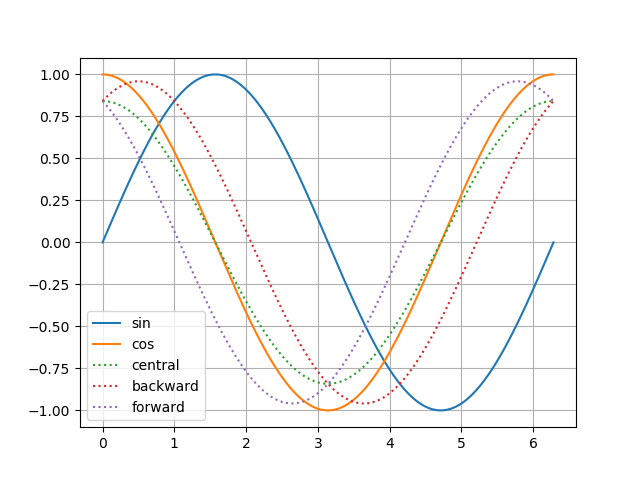
\includegraphics[width=0.7\hsize]{../pics/h=1.png}
  \caption{刻み幅h=1のときの各微分方法の値}
  \label{fig:h_1}
\end{figure}

\begin{figure}[htbp]
  \centering
  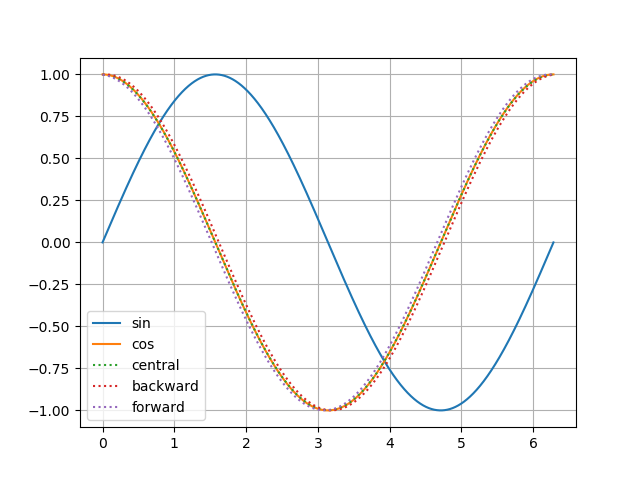
\includegraphics[width=0.7\hsize]{../pics/h=0_1.png}
  \caption{刻み幅h=0.1のときの各微分方法の値}
  \label{fig:h_01}
\end{figure}

$h=1$としたときの前進差分(forward)、後退差分(backward)、中心差分(central)によって
求めた$sin'(x)$の値を図\ref{fig:h_1}に示す。
また、$h=0.1$としたときのものを図\ref{fig:h_01}に示す。

図\ref{fig:h_1}に点線で示された数値微分によって求められた
$sin'(x)$の値は$cos(x)$の値と大きく異なっていることがわかる。
次に、図\ref{fig:h_01}をみるとhが1の時と比べて精度よく求められていることがわかる。
つまり、刻み幅hを小さい値に設定するほど数値微分によって得られた値が
真値(解析的な微分)に近くなると考えられる。

\begin{figure}[htbp]
  \centering
  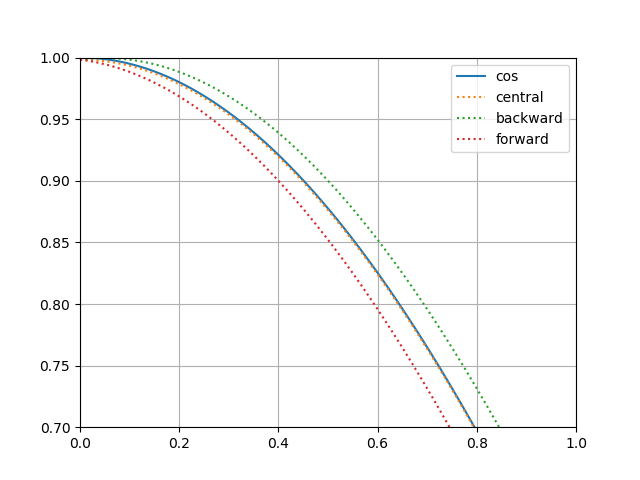
\includegraphics[width=0.7\hsize]{../pics/h=0_1_large.png}
  \caption{h=0.1のときのx=0.5付近での拡大}
  \label{fig:h_01_large}
\end{figure}

\begin{figure}[htbp]
  \centering
  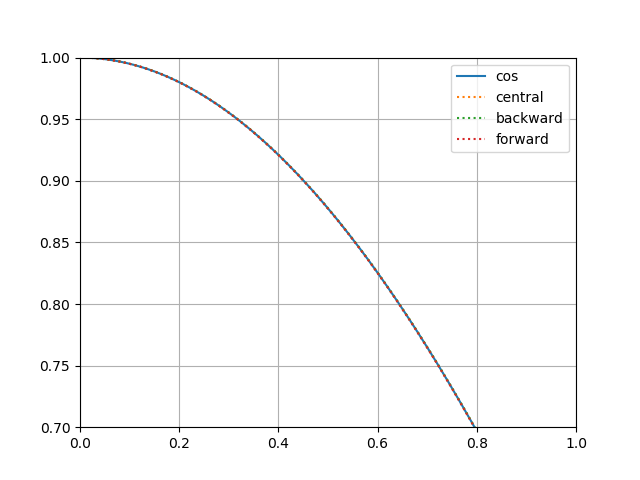
\includegraphics[width=0.7\hsize]{../pics/h=0_001_large.png}
  \caption{h=0.001のときのx=0.5付近での拡大}
  \label{fig:h_0001_large}
\end{figure}

次に、図\ref{fig:h_01_large},\ref{fig:h_0001_large}に、
結果のグラフを拡大したものを示す。
これを見ると、h=0.1であっても前進差分のときは真値より大きく、
後退差分では真値よりも小さい値になってしまっていることがわかる。
しかし、中心差分はほぼ正確に近似できていることがわかる。
中心差分の誤差が前方差分、後方差分よりも小さいことは以下のように証明される。
\begin{eqnarray}
  f(x+h)のテイラー展開\nonumber\\
  f(x+h) ~=~ f(x)+hf'(x)+\frac{h^2}{2!}f''(x)+\frac{h^3}{3!}f'''(x)+O(h^4) \\
  f(x-h)のテイラー展開\nonumber\\
  f(x-h) ~=~ f(x)-hf'(x)+\frac{h^2}{2!}f''(x)+\frac{h^3}{3!}f'''(x)+O(h^4) \\
  中心差分の式\nonumber\\
  \frac{f(x+h)-f(x-h)}{2h} ~&=&~ \frac{2hf'(x)+\frac{2h^3}{3!}f'''(x)+O(h^4)}{2h}\\
  &=&~ f'(x)+O(h^2)
\end{eqnarray}

\begin{figure}[htbp]
  \centering
  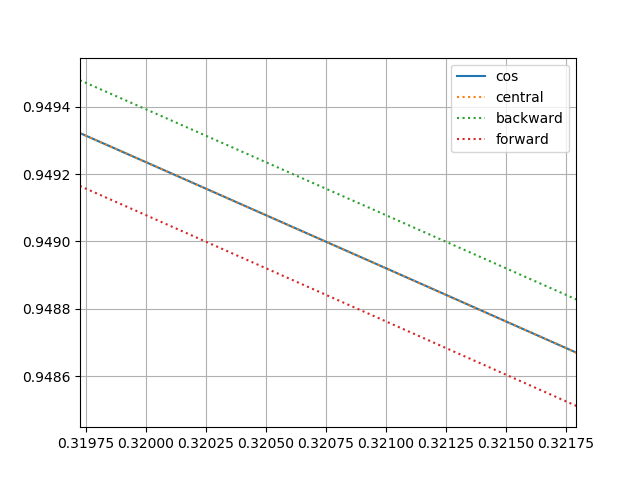
\includegraphics[width=0.7\hsize]{../pics/h=0_001_ll.png}
  \caption{h=0.001の時のものをさらに拡大したもの}
  \label{fig:h_0001_ll}
\end{figure}


\subsection{数値積分によって円の面積を求める}


\subsection{ガウス求積によって円の面積を求める}


\begin{thebibliography}{10}
  \bibitem{1} 台形公式
  \url{https://ja.wikipedia.org/wiki/%E5%8F%B0%E5%BD%A2%E5%85%AC%E5%BC%8F}
  \bibitem{2} シンプソンの公式
  \url{https://ja.wikipedia.org/wiki/%E3%82%B7%E3%83%B3%E3%83%97%E3%82%BD%E3%83%B3%E3%81%AE%E5%85%AC%E5%BC%8F}
  \bibitem{3} ガウス求積
  \url{https://ja.wikipedia.org/wiki/%E3%82%AC%E3%82%A6%E3%82%B9%E6%B1%82%E7%A9%8D}
  \bibitem{数値解析 加古富志雄 令和元年 5 月 27 日}
  \url{https://www.ics.nara-wu.ac.jp/~kako/teaching/na/chap6.pdf}

\end{thebibliography}
\end{document}